
\begin{table}
\renewcommand{\arraystretch}{.75}
\caption{Methods of bird recognition pre-2016.}
\centering
\small
\begin{tabular}{|l|c|c|}
\hline
\textbf{Technique}	&  \textbf{Accuracy} & \textbf{References} \\
\hline
Bayes net			& 69.90 			& \cite{Raghuram2016} \\
SVM 				& 70.75 -- 100 	& \cite{Raghuram2016}\cite{Zhao2017}\cite{Knapp2016} \\
NN 					& 78.60 			& \cite{Raghuram2016} \\
J-48 decision tree 	& 79.60 			& \cite{Raghuram2016} \\
Random forest 		& 83.88 			& \cite{Raghuram2016} \\
Wavelets + NN 		& 78 -- 96 		& \cite{Selin2007} \\
DNN 					& 88.5 -- 95.95	& \cite{Xie2019}\cite{Cakir2017} \\
\hline
\end{tabular}
\end{table}

It convolves a 3D tensor (input, $\mathbf{X}\in \mathbb{R}^{C\times Y\times X}$) with 4D tensors (kernels, $\mathbf{X}\in \mathbb{R}^{N\times C\times H\times W}$) to extract different characteristics, then generates a 3D tensor (output, $\mathbf{Y}\in \mathbb{R}^{C\times Y'\times X'}$) where $C$, $Y$, $X$ are channel, height and width of input tensor, $C$, $H$, $W$ are channel, height and width of one convolution kernel and $N$ is number of convolution kernel, $N$, $Y'$ and $X'$ are channel, height and width of output tensor. Every convolution kernel produces one feature map of output tensor. By default (no padding and stride is one), $X' = X-W+1$ and $Y'=Y-H+1$. For a particular output feature point $(n,y,x)$, 

\[
y(n,y,x) = \sum^C_c\sum^H_j\sum^W_i X(c,y-j,x-i)*W(n,c,j,i)\
\]

\noindent
where $c$, $j$, and $i$ are indices of one of convolution kernels, and $n$ is the n-th convolution kernel. To generate all features, the following algorithm applies:

\begin{figure}[H]
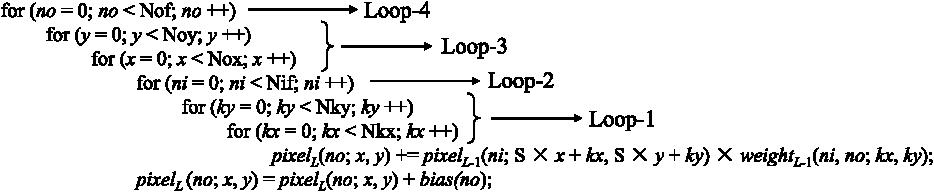
\includegraphics[width=\textwidth]{Ma2018}
\caption{Four levels of convolution loops, where $L$ denotes the index of convolution layer and $S$ denotes the sliding stride. }
\end{figure}

The CONV layer realizes a filter-like process,  which uses a  $K \times K$ weight kernel $W$ to convolve the input feature-map (fmap) $I$ in a sliding-window manner with a stride of $S$. This can be expressed as:

\[
A_n = B(n) + \sum_{m=1}^NW(m,n) \otimes I_m(i,j)
\]

\noindent 
where $\otimes$ is defined as convolution, which equal $K^2$ element-wise multiply-accumulates ($K$ is the kernel size):

\[
X \otimes Y = \sum_{i=1}^K\sum_{j=1}^KX(i,j)\cdot Y(i,j)
\]


Computation of a fully-connected layer can be expressed as matrix multiplication

\[
\mathbf{Y} = \mathbf{W^TX+b}
\]

\noindent 
where $\mathbf{W}\in \mathbb{R}^{M\times N}$ is weights of a fully-connected layer for fusing input features $\mathbf{X}\in \mathbb{R}^M$ to produce output $\mathbf{Y}\in \mathbb{R}^N$. $\mathbf{b}\in \mathbb{R}^N$ is a bias vector to increase non-linearity.


\begin{table}[h]
\renewcommand{\arraystretch}{.75}
\footnotesize
\centering
\caption{Main parameters defining the architectures of the benchmarked CNN networks for 1000-category image recognition \cite{Montero2018}\cite{Hasanpour2016}}
\begin{tabular}{lccccccccc}
\toprule
\textbf{Model}	&	\textbf{MAC}	&	\textbf{CMP}	&	\textbf{ADD}	&	\textbf{DIV}	&	\textbf{ACT}	&	\textbf{Weights}	&	\textbf{Input}	&	\textbf{\# CONV}	&	\textbf{\# FC}	\\
\midrule
SimpleNet	&	1.9G	&	1.82M	&	1.5M	&	1.5M	&	6.38M	&	6.4M	&		&	13	&	1 \\
SqueezeNet	&861.34M	&	9.67M	&	226K	&	1.51M	&	12.58M	&	1.25M	&	224$\times$224$\times$3 &	26	&	0	\\
MobileNet	&			&			&			&			&			&			&	224$\times$224$\times$3	&	27	&	1	\\
ResNet-50	&	3.87G	&	10.89M	&	16.21M	&	10.59M	&	46.72M	&	25.56&	\\
AlexNet		&	7.27G	&	17.67M	&	4.78M	&	9.55M	&	20.81M	&	60.97M	&	224$\times$224$
times$3 \\
\bottomrule
\end{tabular}
\end{table}




\begin{table}[h]
\renewcommand{\arraystretch}{.75}
\centering
\caption{ Summary of weight and MAC number of popular CNNs (\cite{Sze2017}).}
\begin{tabular}{lrrrrr}
\toprule
\textbf{Model} & \textbf{LeNet-5} &  \textbf{AlexNet} & \textbf{VGG-16} & \textbf{GoogLeNet v1} & \textbf{ResNet-50} \\
\midrule
Weights	&	60 K	&	61 M	&	138 M	&	7 M	&	25.5 M \\
MACs	&	341 K	&	724 M	&	15.5 G	&	1.43 G	&	3.9 G \\
\bottomrule
\end{tabular}
\end{table}



\begin{table}
\renewcommand{\arraystretch}{.75}
\centering
\caption{NN for edge.}
\begin{tabular}{lcl}
\toprule
\textbf{Model} & \textbf{Paper} &  \textbf{Contribution} \\
\midrule
MobileNet & \cite{Howard2017} & depthwise separable convolutions \\
ShuffleNet & \cite{Zhang2018}   & depthwise separable convolutions \\
SqueezeNet & \cite{Iandola2017} & Parameter efficiency \\
\bottomrule
\end{tabular}
\end{table}


%\FloatBarrier

\begin{table}
\renewcommand{\arraystretch}{.75}
\small
\centering
\caption{Currently available autonomous sound recorders (\cite{Darras2019}, \cite{Merchant2015}, \cite{Beason2019}). Prices shown include the additional cost of a microphone where one is not provided with the basic unit.}
\label{rpi}
\begin{tabular}{llp{2.5cm}clllllp{2cm}}
\toprule
				&				&						&	&	\multicolumn{2}{c}{\textbf{Power (mW)}}\\
\cline{5-6}
\textbf{Device} & \textbf{Cost} & \textbf{Manufacturer} & \textbf{Storage} & \textbf{Active} & \textbf{Sleep} &  \textbf{Reference} \\
\midrule
SM4BATFS	& \$1099 & Wildlife Acoustics & 512 & 155-270 & 1.8 \\
SM4			& \$1048 & Wildlife Acoustics & 512 & 135-185 & 1.8 \\
Anabat Express & \textsterling 834 & Titley Scientific & 32 & 69-113 & 3.1 \\
RPA2 		& \textsterling 210 & Peersonic & 32 & 405-605 & 30 \\
Solo 		& \textsterling 63 & $\dagger$ & 256 & 315-450 & -- &  \cite{Whytock2017} \\
Audiomoth 	& \textsterling 36 & Open Acoustic Devices & 32 & 17-70 & 0.08 & \cite{Hill2018} \\
%Bat Pi 2 & -- & Fledermausschutz & 64 & -- & -- & \cite{Fledermausschutz2015} \\
Swift && Cornell & \\
-- & &Imperial College &&&& \cite{Sethi2018} \\
\bottomrule
\end{tabular}
\newline
$\dagger$ Open source
\end{table}



In automatic bioacoustic monitoring it is important to do continuous observations to capture rare events, but storage and communication overheads typically prevent continuous real- time monitoring. To overcome this limitation, this paper presents a low complexity local processing method for acoustic signals targeting resource constrained nodes and preprocessing and seg- mentation techniques in line with the proposed local processing technique for effective and continuous identification of bird calls. This paper also focuses on designing of overall automatic bioacoustic monitoring system including feature extraction and classification.
(\cite{Weerasena2019})

FPGA-based feature extraction implementation allows the system to process data from 30 acoustic sensors in real time with.
In terms of the implementation of the birdsong recognition system, the Mel scale filter bank entails the highest execution cost. Since the series implementation still shows acceptable results in terms of time consumption %\cite{Hervas2017}

Automated Remote Biodiversity Monitoring Network (ARBIMON), a novel combination of hardware and software for automating data acquisition, data management, and species identification based on audio recordings. The major components of the cyberinfrastructure include: a solar powered remote monitoring station that sends 1-min recordings every 10 min to a base station, which relays the recordings in real-time to the project server, where the recordings are processed and uploaded to the project website (arbimon.net). (\cite{Aide2013})


\begin{figure}[ht]
\centering
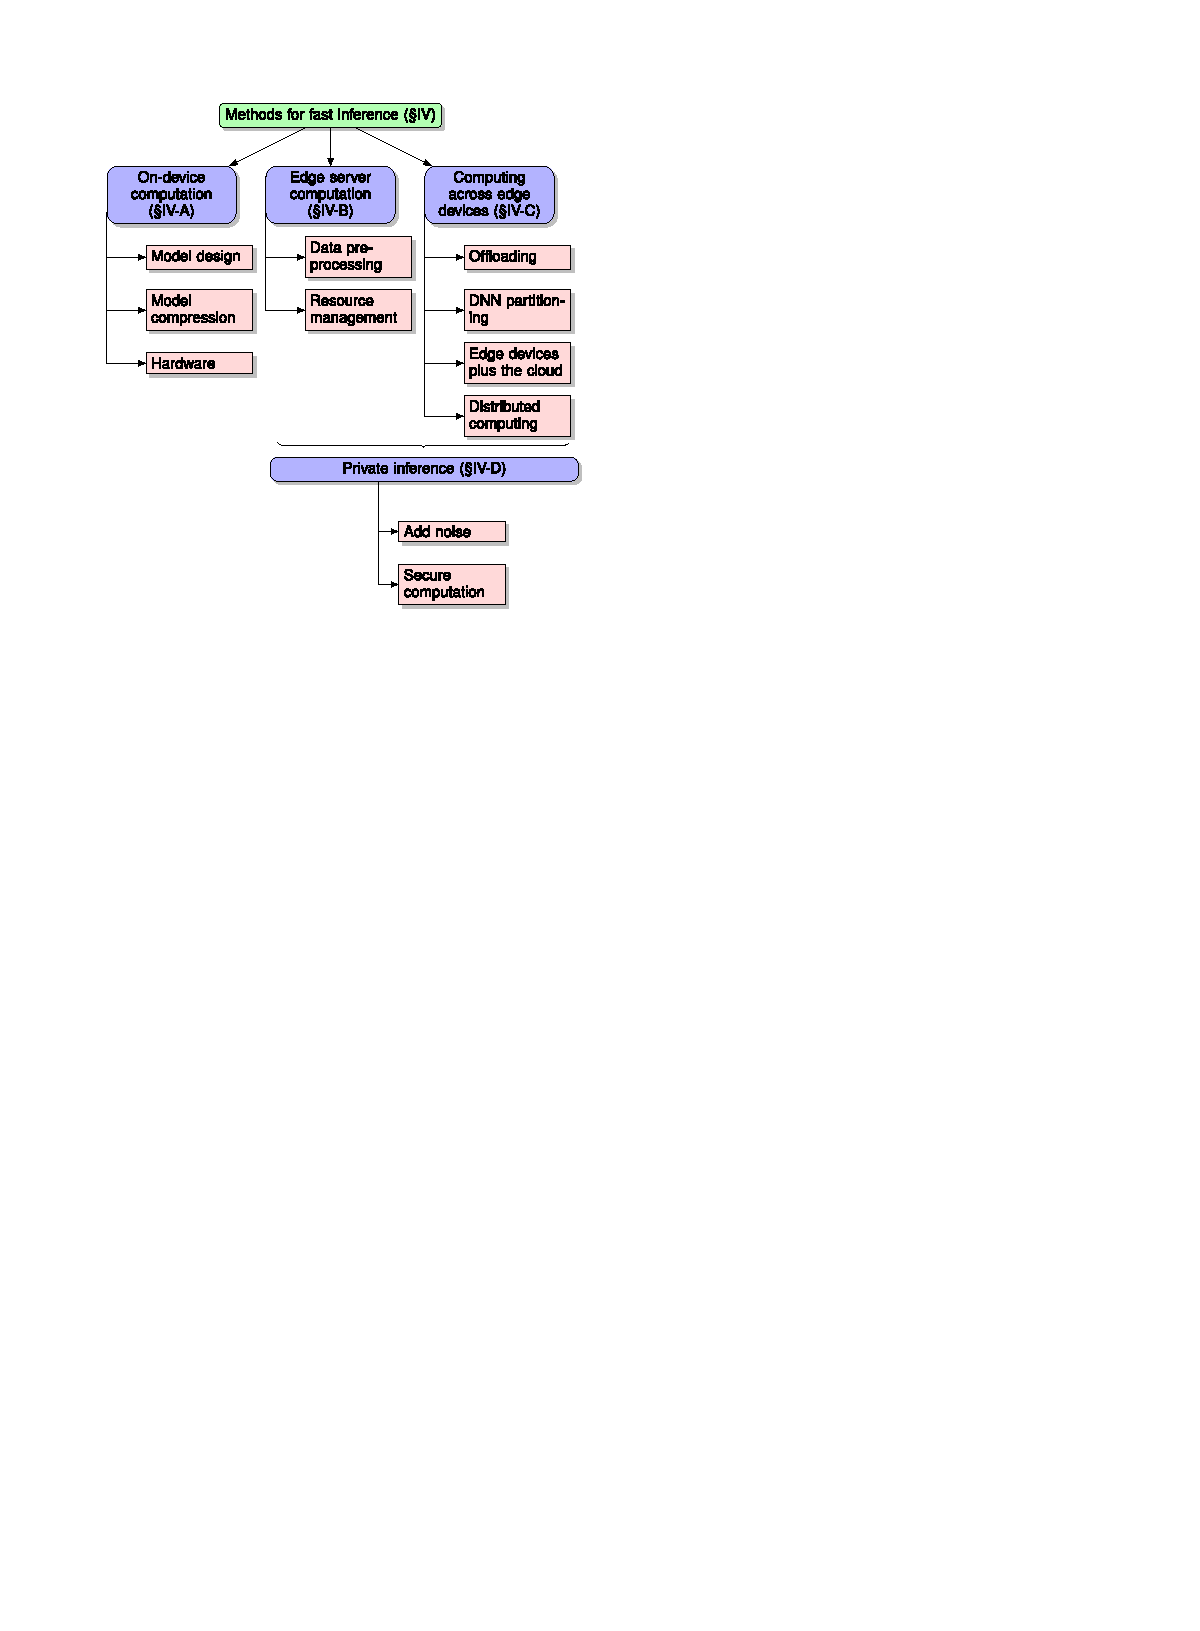
\includegraphics[scale=1.2]{chen2019methodsfastinference}
\caption{Methods for fast edge inference (\cite{Chen2019}).}
\end{figure}

While there has been extensive investigation on reducing the complexity of well studied CNN models in the form of parameter compression and quantization, there has been limited effort on developing specialized CNN designs for bird species classification. 
As such, in this work we focus on designing an efficient and lightweight network to accelerate the execution of the model with minimal compromise on the achieved accuracy

First, we adapted this basic model to detect only one class. Second, we explore the impact on performance by changing the structure of a CNN network such as the number of filters, the number of layers, the image size, the number of convolution and the pooling layers. Overall we design .... different structures



\begin{table}
\small
\centering
\caption{Bioacoustic detection algorithms.}
\label{biodetect}
\begin{tabular}{lll}
\toprule
Algorithm & Platform & Ref \\
\midrule
Goetzel filter & Audiomoth & \cite{Prince2019} \\
Bat detective & i9 & \cite{MacAodha2018} \\
\bottomrule
\end{tabular}
\end{table}

